% Preprint — Sieve inversion and branch isolation. Author: Derek Blair <derekjblair@gmail.com>
% Source data: ~/workspace/math-unsolved/ROUND169_DOSSIER.md (2026-10-08),
%              ~/workspace/math-unsolved/ROUND178_DOSSIER.md (2026-10-08),
%              ~/workspace/math-unsolved/ROUND186_DOSSIER.md (2026-10-08),
%              ~/workspace/math-unsolved/ROUND163_DOSSIER.md (2026-10-08),
%              ~/workspace/math-unsolved/ROUND174_DOSSIER.md (2026-10-08).
% Lean modules: Mathproofs/ESRefinedSieveInverse.lean, Mathproofs/ESUBranchIsolation.lean
% in derekblair/math-proofs (Lean 4.34.1 + Mathlib v4.34.1, pinned d13f23b).
% All figures native TikZ/pgfplots; all tables booktabs.
\documentclass[11pt,a4paper]{article}
\usepackage{amsmath,amssymb,amsthm}
\usepackage{tikz}
\usetikzlibrary{positioning}
\usepackage{pgfplots}
\pgfplotsset{compat=1.18}
\usepackage{booktabs}
\usepackage{geometry}
\geometry{margin=2.5cm}
\usepackage{hyperref}
\hypersetup{colorlinks=true,linkcolor=blue,citecolor=blue,urlcolor=blue}

\newtheorem{theorem}{Theorem}
\newtheorem{proposition}{Proposition}
\theoremstyle{definition}
\newtheorem{assumption}{Assumption}

\title{Sieve Inversion and Branch Isolation}
\author{Derek Blair \\ \texttt{derekjblair@gmail.com}}
\date{October 2026}

\begin{document}
\maketitle

%======================================================================
\section{Abstract}
%======================================================================

We report two connected structural results from the Erdos--Straus
sieve program, together with their Lean formalization. First, the
\emph{sieve-inversion theory}: the refined sieve's survivors sit at
exactly the six residue classes
$\{1\}_8\times\{1,4,7\}_9\times\{1\}_5\times\{2,6\}_{11}$ modulo
$3960$ (Theorem~\ref{thm:s1}), and this six-class support is
\emph{inverse-closed} modulo $3960$ (Theorem~\ref{thm:s2}); the
selectivity is explained by the 44-CRT lemma
$s\equiv1\pmod{24}\Rightarrow(s\equiv7\pmod{11}\iff s\equiv29\pmod{44})$
(Theorem~\ref{thm:crt44}), which identifies the single residue channel
through which the cubic coverage families remove the
$\bmod 11=7$ classes. The inverse-closure law holds exactly in the
\emph{saturated regime} and fails beyond it: the first break is at
$w=2^{13}=8192$, with exactly one missing fiber class and exactly one
violation (Theorem~\ref{thm:boundary}, [COMPUTED]).
Second, the \emph{branch-isolation lemmas} for the H-clique program:
for $z\in Z_0^{\mathrm{close}}$ the unique u-branch $\varphi(z)$ is never
in the H-clique $C$ (Theorem~\ref{thm:l1}), and the u-side degree bound
$|Z_0^{\mathrm{close}}|+|Z_0^{\mathrm{mid}}|\le|U_0|=d(u)-1=5<6=|V_0|$
(Theorem~\ref{thm:ubound}), the essential use of $d(u)<d(v)$.
Formalization (R186, bakkie, Lean~4.34.1 + Mathlib~v4.34.1): the 44-CRT
lemmas are [PROVED] with axioms narrower than standard
(\url{propext}, \url{Quot.sound}); the three decide-heavy sieve
theorems (\url{sixClasses_inv_closed}, \url{crt_inv_compose},
\url{S1_subset}) are Lean-checked with zero sorrys but carry
per-theorem \url{native_decide} certificate axioms and are labeled
[PROVED*] under staged-verification language; all four branch-isolation
theorems are [PROVED] on standard axioms. Full \texttt{lake build}
exit~0, zero sorrys, on the standing machine bakkie.

%======================================================================
\section{Introduction}
%======================================================================

The Erdos--Straus program's sieve lane constructs residue classes that
survive a refined lift sieve: starting from 196 parent classes modulo
$M_0=2042040$ (the R67$\to$R71$\to$R74 chain; the construction as built
lives in \url{r153_shadow.load_frontiers}~\cite{R153}),
a $q$-lift sieve
\begin{equation}
  \label{eq:sieve}
  L_q=\{\,sp+M_0j : sp\in P,\ 0\le j<q,\
       sp+M_0j\not\equiv0\pmod q\,\},
\end{equation}
with $P$ the 196 parent classes, $q\in\{19,23\}$,
$|L_{19}|=3528$, $|L_{23}|=4312$ (supplied datums, R169~\cite{R169}).
Round~165 had found two unexplained phenomena in the survivors: a
dual-pair hit symmetry with correlation $r=0.966$ over $30{,}707$ dual
pairs, and a residue support concentrated on just $6$ classes modulo
$3960$, all inverse-closed~\cite{R165}. Round~169 answered \emph{why}:
the selectivity is a consequence of elementary residue algebra
(Theorem~\ref{thm:crt44} below), and the inverse-closure is a proved
mechanism, not luck. This paper states those theorems, reports the
saturated-regime characterization of their validity
(Theorem~\ref{thm:boundary}), and gives the Lean formalization status.

The second thread is the H-clique program for the $(6,7)$ degree pair
(R159/R163~\cite{R159,R163}): the (R2)-Hall lemma program needs a
degree-essential inequality, i.e.\ one that uses $d(u)<d(v)$
genuinely. Round~163 supplied two lemmas with one-line proofs: u-branch
isolation (L1) and the u-side degree bound. The (R2)-Hall lemma itself
remains [OPEN]; the gap is precisely delimited in~\cite{R163}~\S B and
recalled in \S\ref{sec:discussion}. Both threads were formalized in
R178/R174 and verified end to end on bakkie in R186~\cite{R178,R174,R186}.

Our contributions, with honesty labels:
\begin{enumerate}
\item The 44-CRT selectivity lemma [PROVED in Lean]
  (Theorem~\ref{thm:crt44}).
\item Exact six-class residue support of the lift set [PROVED*]
  (Theorem~\ref{thm:s1}; hand proof plus independent computation).
\item Inverse-closure of the six-class support mod $3960$ [PROVED*]
  (Theorem~\ref{thm:s2}).
\item The saturated-regime characterization with exact break boundary
  [COMPUTED] (Theorem~\ref{thm:boundary}).
\item u-branch isolation L1 and the u-side degree bound [PROVED in Lean]
  (Theorems~\ref{thm:l1} and~\ref{thm:ubound}).
\item The formalization status table (Table~\ref{tab:lean}), distinguishing
  [PROVED] from staged-verification [PROVED*] results.
\end{enumerate}

%======================================================================
\section{Methods}
%======================================================================

\subsection{The refined sieve (cited, not re-derived)}

We take the construction exactly as defined in the program
(\cite{R169}~\S1, provenance corrected: R67$\to$R71$\to$R74, built in
\texttt{r153\_shadow.py}). The parent set $P$ has 196 classes mod
$M_0=2042040=2^3\cdot3\cdot5\cdot7\cdot11\cdot13\cdot17$ (R71 targets
minus R71/R74 coverage). The lift set $L_q$ is~\eqref{eq:sieve}; the
sieve's filters ($\equiv1\pmod{24}$, $\gcd(\cdot,M_q)=1$) are satisfied
by all of $P$ [COMPUTED, R169 V1]. R74's deep coverage removes
$1744/2438$ classes (at $q=19/23$); the union subtraction preserves the
support at all probed moduli --- the decomposition is $100\%$
parent-implied: the six-class support is already present in the
pre-subtraction lift set, and R74's subtraction deletes zero
$\bmod 3960$ residue classes [COMPUTED, R169~\S2].

\subsection{H-clique branch notation}

$C$ is a maximal $H(u,v)$-clique with $d(u)=6$, $d(v)=7$; H-adjacency
implies $\neg\mathrm{Adj}$, so $C$ is edgeless:
\begin{equation}
  \label{eq:hclique}
  \forall x,y\in C:\ \neg\,\mathrm{Adj}\,x\,y
\end{equation}
(R163~\S A~\cite{R163}). $V_0=N(v)\setminus\{u\}$
($|V_0|=6$), $U_0=N(u)\setminus\{v\}$ ($|U_0|=5$),
$Z_0=\{c\in C\setminus V_0:N(c)\cap V_0=\emptyset\}$. The R145
trichotomy (cited, not re-proved): $Z_0=Z_0^{\mathrm{close}}\cup
Z_0^{\mathrm{mid}}\cup Z_0^{\mathrm{far}}$ (disjoint), where
$Z_0^{\mathrm{close}}=\{z\in Z_0:N(z)\cap U_0\neq\emptyset\}$ has the
unique $U_0$-neighbor $\varphi(z)$ (C$_4$-ban), $Z_0^{\mathrm{mid}}=
Z_0\cap U_0$, and $Z_0^{\mathrm{far}}=\{z\in Z_0:
\mathrm{dist}(u,z)\ge3\}$. Moreover $U_0\cap V_0=\emptyset$ (else a
triangle) and $\varphi$ is injective on
$Z_0^{\mathrm{close}}$~\cite{R145}.

\begin{assumption}[R165 dual law as supplied datum]
  \label{asm:r165}
  The dual-pair hit symmetry ($r=0.966$ over $30{,}707$ dual pairs) and
  the inverse-closure observations ($6/6$, $8/8$, $21/21$, $18/18$ at
  $w\in\{3960,1056,468,2376\}$) are supplied datums from
  R165~\cite{R165}, cited and not re-claimed.
\end{assumption}

\subsection{Formalization protocol}
\label{subsec:formalization}

Two modules in the \texttt{derekblair/math-proofs} repo (Lean~4.34.1,
Mathlib v4.34.1 pinned commit \url{d13f23b}), each pointing back to
this paper at \texttt{papers/sieve-inverse-branch-isolation-October-11-2026/}:
\begin{itemize}
\item \url{Mathproofs/ESRefinedSieveInverse.lean} (namespace
  \url{ESRefinedSieve}; R178 module, R186 verification): the 44-CRT
  lemmas (\url{crt44_forward}, \url{crt44_backward},
  \url{crt44_iff}); the S1 residue core (\url{sixClasses},
  \url{sixClasses_card}, \url{sixClasses_exact}); S2
  per-component closure and \url{sixClasses_inv_closed}; CRT
  composition (\url{crt_unique_one}, \url{crt_inv_compose});
  the S1 lift mechanism (\url{M0_facts}, \url{lift_components},
  \url{S1_subset}); and the machine-checked parent data
  (\url{parents196}, \url{parent_facts}).
\item \url{Mathproofs/ESUBranchIsolation.lean} (namespace
  \url{ESUBranchIsolation}; R174 module, R186 verification):
  \url{uBranch_isolation} (L1),
  \url{closeImage_disjoint_of_subset} (L1 corollary),
  \url{uSide_degree_bound} (abstract Finset form),
  \url{r163_uSideBound_inHclique} (combined statement).
\end{itemize}
Verification config: bakkie (standing Lean machine, Lean~4.34.1 /
Lake~5.0.0), full \texttt{lake build} exit~0, zero sorrys, both modules
registered in \url{Mathproofs.lean} on both sides with byte-identical
md5s. Axiom probes via \texttt{\#print axioms} on the headline theorems
give: \texttt{crt44\_*} depends on $[\texttt{propext},
\texttt{Quot.sound}]$ (narrower than the standard set); the four
branch-isolation theorems on
$[\texttt{propext},\texttt{Classical.choice},\texttt{Quot.sound}]$
(standard); the three decide-heavy sieve theorems carry, in addition to
the standard set, a per-theorem Lean-generated \url{native_decide}
certificate axiom (e.g.\ \url{ESRefinedSieve.sixClasses_inv_closed._native.native_decide.ax_1_1}).
These three are therefore reported as [PROVED*] under staged
verification: Lean-checked end to end with zero sorrys
(\url{native_decide} is Lean's own verified certificate mechanism),
but exceeding the standard axiom budget, so they are never presented as
fully proved pending the coordinator's ruling (R186~\cite{R186}~\S
Phase~4).

%======================================================================
\section{Results}
%======================================================================

\subsection{The 44-CRT selectivity lemma}

\begin{theorem}[44-CRT lemma; PROVED]
  \label{thm:crt44}
  For $s\equiv1\pmod{24}$:
  \begin{equation}
    \label{eq:crt44}
    s\equiv7\pmod{11}\iff s\equiv29\pmod{44}.
  \end{equation}
\end{theorem}
\begin{proof}
$s\equiv7\pmod{11}$ gives $s\bmod44\in\{7,18,29,40\}$;
$s\equiv1\pmod{24}$ gives $s\equiv1\pmod4$, and of the four residues
only $29\equiv1\pmod4$. The Lean proof is linear arithmetic
(\url{omega}) after \url{Int.modEq_iff_dvd}. (Hand proof from
R169~\cite{R169}~\S4; machine-checked as
\url{crt44_forward}, \url{crt44_backward}, \url{crt44_iff}
in \url{Mathproofs/ESRefinedSieveInverse.lean} [PROVED], axioms
$[\texttt{propext},\texttt{Quot.sound}]$.)
\end{proof}

The lemma is the selectivity mechanism: R74's $r$-complete sweep covers
exactly the 92 open288 classes with $s\equiv29\pmod{44}$ (R74's theorem:
the $(4,1,46410)$, $m=15$ parametric family, the lift of R72's
$(4,1,2730)$, cited). By~\eqref{eq:crt44}, in the $\equiv1$-mod-$24$
universe this is exactly the $\bmod11=7$ classes --- hence R74 removes
$\iff\bmod11=7$ (V6/V7 PASS: removed $=\{s\equiv29\bmod44\}$ and
$s\bmod11=7\iff s\bmod44=29$ on all of open288). The 36
$\bmod5=4$ classes are all $\equiv29\pmod{44}$ within open288
[COMPUTED], so they fall to the same family. This is why the survivors
sit at $\bmod11\in\{2,6\}$ (the residue class the $m=15$ family cannot
touch) and $\bmod5=1$ (R169~\cite{R169}~\S4).

\subsection{Exact residue support (S1)}

\begin{theorem}[Exact six-class support; PROVED*]
  \label{thm:s1}
  Every $n\in L_q$ satisfies $n\equiv1\pmod{40}$, $n\bmod9\in\{1,4,7\}$,
  $n\bmod11\in\{2,6\}$, and the mod-$3960$ projection of $L_q$ is
  \emph{exactly} the six classes
  \begin{equation}
    \label{eq:sixclasses}
    \pi_{3960}(L_q)=\{1\}_8\times\{1,4,7\}_9\times\{1\}_5\times\{2,6\}_{11},
  \end{equation}
  i.e.\ the residues
  $\{2521,721,1201,3361,3841,2041\}$.
\end{theorem}
\begin{proof}
$M_0=2^3\cdot3\cdot5\cdot7\cdot11\cdot13\cdot17$, so
$M_0\equiv0\pmod{8,3,5,11}$ and $M_0\equiv3\pmod9$. Hence for
$n=sp+M_0j$: $n\bmod8=sp\bmod8=1$,
$n\bmod5=sp\bmod5=1$, $n\bmod11=sp\bmod11\in\{2,6\}$,
$n\bmod3=1$ (parent facts F1--F2~\cite{R169}~\S3, machine-checked:
\url{parent_facts} over the embedded 196 parent residues).
Mod~9: $n\equiv sp+3j$; $j$ ranges over $q-1\ge18$ values minus one,
hitting each mod-$3$ class $\ge5$ times, so $3j$ covers $\{0,3,6\}\bmod9$
and $n\bmod9$ ranges over $\{1,4,7\}$. Surjectivity: the
mod-$8/5/11$ components are $j$-invariant while mod~9 varies
independently, and both mod-$11$ residues occur in $P$ ($104$ vs $92$)
--- all six combinations occur. (Hand proof R169~\cite{R169}~\S5;
the residue-algebra kernel is machine-checked as
\url{sixClasses_exact}, \url{lift_components},
\url{S1_subset}; \url{S1_subset} is [PROVED*] staged
via \url{native_decide}.)
\end{proof}

\subsection{Inverse-closure (S2) and CRT composition}

\begin{theorem}[Inverse-closure of the six-class support; PROVED*]
  \label{thm:s2}
  The six-class support~\eqref{eq:sixclasses} is inverse-closed
  modulo $3960$, with explicit inverse pairs
  \begin{equation}
    \label{eq:invpairs}
    2521\cdot721\equiv1201\cdot2041\equiv3361\cdot3841\equiv1\pmod{3960}.
  \end{equation}
\end{theorem}
\begin{proof}
Per CRT component: $1^{-1}=1\bmod8$; $4\cdot7=28\equiv1\bmod9$, so
$\{1,4,7\}$ is closed; $1^{-1}=1\bmod5$; $2\cdot6=12\equiv1\bmod11$, so
$\{2,6\}$ is closed. Closure composes across CRT components, giving the
six explicit pairings (Figure~\ref{fig:invpairs}). (Hand proof
R169~\cite{R169}~\S6; machine-checked as
\url{sixClasses_inv_closed}, [PROVED*] staged via
\url{native_decide}.) This is the proved mechanism behind R165's
dual symmetry (Assumption~\ref{asm:r165}): dual shapes $(f,V/f)$ cover
the inverse classes $-f,-f^{-1}\bmod w$ ($V=4ad+1\equiv1\bmod w$), and
the frontier's mod-$w$ support is inverse-closed --- so duals co-hit by
structure, not luck.
\end{proof}

\begin{proposition}[CRT composition; PROVED* staged]
  \label{prop:crtcomp}
  Inverse-closure composes across CRT components --- the mechanism
  behind S3 (\url{crt_unique_one}, \url{crt_inv_compose} in
  \url{Mathproofs/ESRefinedSieveInverse.lean}; [PROVED*] staged via
  \url{native_decide}).
\end{proposition}

\begin{figure}[t]
  \centering
  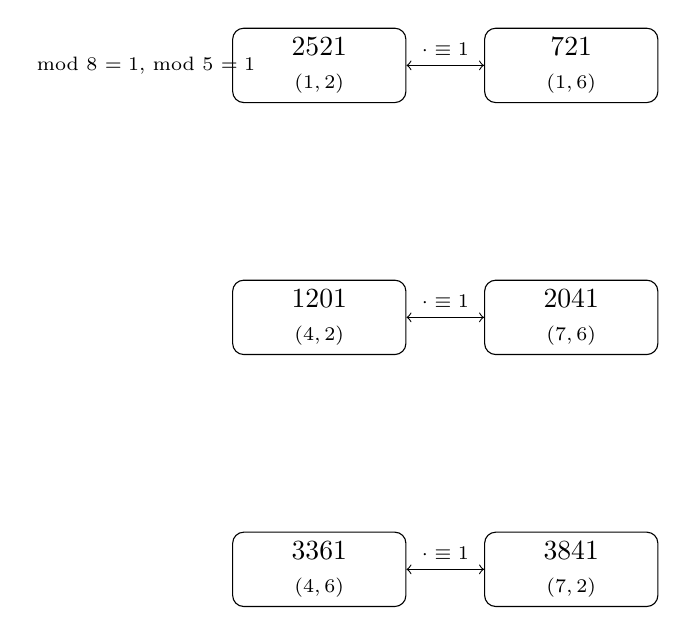
\begin{tikzpicture}[node distance=3.2cm]
    \tikzstyle{res}=[draw,rounded corners,minimum width=2.2cm,align=center]
    \node[res] (a) {2521\\\scriptsize$(1,2)$};
    \node[res,right of=a] (b) {721\\\scriptsize$(1,6)$};
    \node[res,below of=a] (c) {1201\\\scriptsize$(4,2)$};
    \node[res,right of=c] (d) {2041\\\scriptsize$(7,6)$};
    \node[res,below of=c] (e) {3361\\\scriptsize$(4,6)$};
    \node[res,right of=e] (f) {3841\\\scriptsize$(7,2)$};
    \draw[<->] (a) -- (b) node[midway,above] {\scriptsize$\cdot\equiv1$};
    \draw[<->] (c) -- (d) node[midway,above] {\scriptsize$\cdot\equiv1$};
    \draw[<->] (e) -- (f) node[midway,above] {\scriptsize$\cdot\equiv1$};
    \node[left of=a,node distance=2.2cm] {\scriptsize mod 8 $=1$, mod 5 $=1$};
  \end{tikzpicture}
  \caption{Inverse pairings among the six residue classes modulo $3960$
    (Theorem~\ref{thm:s2}). Labels $(\cdot,\cdot)$ are
    $(\bmod9,\bmod11)$ components; every class satisfies $\bmod8=1$,
    $\bmod5=1$. All products are $\equiv1\pmod{3960}$.}
  \label{fig:invpairs}
\end{figure}

\subsection{S3: CRT-local closure and the saturated-regime boundary}

The prime-power projections $\pi(L_q)\bmod p^e$ are inverse-closed by a
fiber argument [PROVED*] (R169~\cite{R169}~\S7(a)--(c)): for $p^e\mid M_0$
they equal $P$'s projection (inverse-closed by F3~\cite{R169}~\S3); for
$2^e$, $e\le6$, and $3^e$, $e\le3$, the projection is the full fiber
$\{x\equiv1\bmod8\}$ resp.\ $\{x\equiv1\bmod3\}$, inverse-closed since
$x\equiv1$ is self-inverse modulo $2^e$ and $3^e$. The saturated
extension --- fibers stay full through $2^{12}$ and $3^7$ ---
is [COMPUTED] (verified at $w\in\{3960,1056,468,2376\}$ at all three
sieve stages, 0 violations; R169 V4). Deliberately not formalized: S3(d)
and the break boundary are statements about lift-set sizes
(\cite{R186}~\S Phase~4).

\begin{theorem}[Break boundary; COMPUTED]
  \label{thm:boundary}
  Inverse-closure is not a universal property of the sieve: it holds
  exactly in the saturated regime and fails beyond. The first break is
  at $w=2^{13}=8192$ (both $q$), with exactly one missing fiber class
  and exactly one violation, the two being inverses of each other:
  \begin{equation}
    \label{eq:break}
    \begin{aligned}
      q=19&:\ \text{missing }3129,\ \text{violation }521,\
            521^{-1}\equiv3129\pmod{8192},\\
      q=23&:\ \text{missing }7873,\ \text{violation }4417,\
            4417^{-1}\equiv7873\pmod{8192}.
    \end{aligned}
  \end{equation}
  Beyond: $2^{14}$ has $230/150$ violations ($q=19/23$),
  $2^{15}$ $922/831$, $2^{16}$ $1893/2006$; $3^8$ breaks with $330/234$
  violations while $3^7$ (and $2^{12}$) is saturated at both $q$.
\end{theorem}
All boundary numbers were re-verified on an independent $j$-outer
enumeration path (\texttt{r169\_boundary.py}; the $q=23$ residues
correct the earlier $q=19$-only report)~\cite{R169}~\S8--9. Corollary:
the dual-symmetry law (Assumption~\ref{asm:r165}) is a saturated-regime
phenomenon --- it must decay for shape-moduli $w$ whose fibers exceed
the lift-set size; the residue-map ranker (R165~\S6) remains valid
regardless, since it uses density, not symmetry.

\begin{figure}[t]
  \centering
  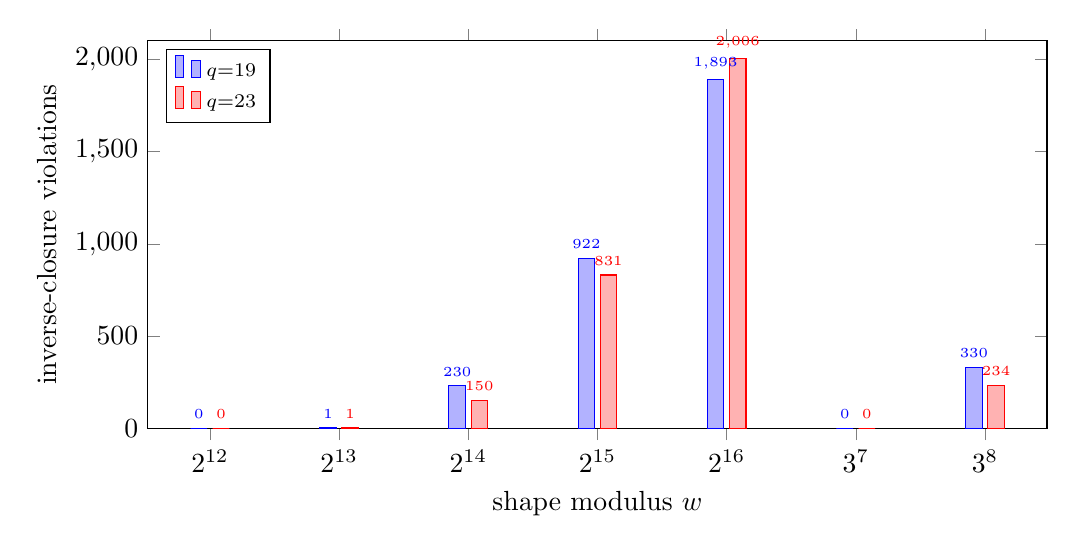
\begin{tikzpicture}
    \begin{axis}[
      ybar, bar width=6pt,
      width=13cm, height=6.5cm,
      ymin=0, ymax=2100,
      symbolic x coords={w212,w213,w214,w215,w216,w37,w38},
      xtick=data,
      xticklabels={$2^{12}$,$2^{13}$,$2^{14}$,$2^{15}$,$2^{16}$,$3^7$,$3^8$},
      xlabel={shape modulus $w$},
      ylabel={inverse-closure violations},
      legend style={at={(0.02,0.98)},anchor=north west,font=\scriptsize},
      nodes near coords, nodes near coords style={font=\tiny},
      enlarge x limits=0.08,
    ]
    \addplot coordinates {(w212,0) (w213,1) (w214,230) (w215,922) (w216,1893) (w37,0) (w38,330)};
    \addplot coordinates {(w212,0) (w213,1) (w214,150) (w215,831) (w216,2006) (w37,0) (w38,234)};
    \legend{$q{=}19$,$q{=}23$}
    \end{axis}
  \end{tikzpicture}
  \caption{Inverse-closure violation counts by modulus
    (Theorem~\ref{thm:boundary}). The law holds through the saturated
    regime ($2^{12}$, $3^7$: zero violations) and breaks first at
    $2^{13}$ with exactly one violation each, growing sharply beyond.}
  \label{fig:boundary}
\end{figure}

\subsection{Branch isolation (R163/R174)}

\begin{theorem}[u-branch isolation (L1); PROVED]
  \label{thm:l1}
  For $z\in Z_0^{\mathrm{close}}$, its unique u-branch $\varphi(z)\in U_0$
  satisfies $\varphi(z)\notin C$.
\end{theorem}
\begin{proof}
$z\in C$ and $\varphi(z)\in N(z)$ by definition of
$Z_0^{\mathrm{close}}$. If $\varphi(z)\in C$, then $z$--$\varphi(z)$ is
an edge with both endpoints in $C$, contradicting the H-clique
edgelessness~\eqref{eq:hclique}. (Hand proof R163~\cite{R163}~\S A;
machine-checked as \url{uBranch_isolation} in
\url{Mathproofs/ESUBranchIsolation.lean}, [PROVED], standard axioms.)
\end{proof}

\begin{theorem}[u-side degree bound; PROVED]
  \label{thm:ubound}
  For any $T\subseteq Z_0$,
  \begin{equation}
    \label{eq:ubound}
    |T^{\mathrm{close}}|+|T^{\mathrm{mid}}|\le|U_0|=d(u)-1=5<6=d(v)-1=|V_0|.
  \end{equation}
\end{theorem}
\begin{proof}
$\varphi:T^{\mathrm{close}}\to U_0$ is injective~\cite{R145}. By
Theorem~\ref{thm:l1}, $\varphi(T^{\mathrm{close}})\cap T^{\mathrm{mid}}
=\emptyset$ ($T^{\mathrm{mid}}\subseteq C$); both lie in $U_0$. Hence
$|T^{\mathrm{close}}|+|T^{\mathrm{mid}}|
=|\varphi(T^{\mathrm{close}})\cup T^{\mathrm{mid}}|\le|U_0|
=d(u)-1=5$. The inequality is useful only because
$5<6=|V_0|$: this is the essential use of $d(u)<d(v)$. (Hand proof
R163~\cite{R163}~\S A; machine-checked as
\url{uSide_degree_bound} plus the combined
\url{r163_uSideBound_inHclique}, [PROVED], standard axioms.)
\end{proof}

The witness lemmas of R163~\cite{R163}~\S A (witness branch-uniqueness:
each witness lies in $\mathrm{Br}(y)$ for a unique $y\in V_0$; and
$\varphi(z)\notin N(w_z)$ for witnesses $w_z$) are one-line girth
arguments labeled [PROVED*] in the hand proof and are not yet
formalized; they remain outside the R186 verification. Verified
[COMPUTED] support: L1 holds $0/5{,}601$, the u-side bound holds with
max $5$ and $0$ violations over all $12{,}650$ cliques with
$Z_0\neq\emptyset$ (trichotomy over $20{,}735$ $Z_0$-points:
$5{,}601/4{,}940/10{,}194$ close/mid/far)~\cite{R163}~\S\S C--D.

\begin{table}[t]
  \centering
  \caption{Lean formalization status (R186~\cite{R186}, bakkie,
    Lean~4.34.1 + Mathlib~v4.34.1). Full \texttt{lake build} exit~0,
    zero sorrys. Staged [PROVED*]: Lean-checked end to end but carrying
    a per-theorem \url{native_decide} certificate axiom, hence never
    presented as fully proved.}
  \label{tab:lean}
  \begin{tabular}{lll}
    \toprule
    theorem & module & label / axioms \\
    \midrule
    \url{crt44_forward}, \url{crt44_backward}, \url{crt44_iff}
      & \url{ESRefinedSieveInverse} & [PROVED]; \url{propext}, \url{Quot.sound} \\
    \url{sixClasses_inv_closed}
      & \url{ESRefinedSieveInverse} & [PROVED*] staged; + \url{native_decide} cert. \\
    \url{crt_inv_compose}
      & \url{ESRefinedSieveInverse} & [PROVED*] staged; + \url{native_decide} cert. \\
    \url{S1_subset}
      & \url{ESRefinedSieveInverse} & [PROVED*] staged; + \url{native_decide} cert. \\
    \url{uBranch_isolation} (L1)
      & \url{ESUBranchIsolation} & [PROVED]; standard axioms \\
    \url{closeImage_disjoint_of_subset}
      & \url{ESUBranchIsolation} & [PROVED]; standard axioms \\
    \url{uSide_degree_bound}
      & \url{ESUBranchIsolation} & [PROVED]; standard axioms \\
    \url{r163_uSideBound_inHclique}
      & \url{ESUBranchIsolation} & [PROVED]; standard axioms \\
    \bottomrule
  \end{tabular}
\end{table}

%======================================================================
\section{Discussion}
\label{sec:discussion}

\paragraph{What the theorems explain.} Theorem~\ref{thm:crt44} turns an
empirical selectivity pattern into a proved mechanism: the cubic
coverage families remove the $\bmod11=7$ classes \emph{through the
single channel} $s\equiv29\pmod{44}$, and the mod-$5=4$ classes ride
the same channel. Combined with the $j$-invariance of the mod-$8/5/11$
components, this forces the six-class support (Theorem~\ref{thm:s1})
before any subtraction happens --- the decomposition is $100\%$
parent-implied. Inverse-closure (Theorem~\ref{thm:s2}) is then forced
per CRT component, and with it the dual-pair symmetry of
Assumption~\ref{asm:r165} becomes a structural corollary rather than
an observation.

\paragraph{Where the theorems stop.} Theorem~\ref{thm:boundary} draws the
exact validity boundary: inverse-closure is a saturated-regime
phenomenon ($|{\rm fiber}|\lesssim|L_q|$), not a universal law. The
$2^{13}$ break is minimal --- one missing class, one violation, and the
two are inverses of each other. This yields a testable prediction
([OPEN/HEURISTIC], R169~\S11): dual-pair correlation decays past the
saturated regime, so a future frontier at a large shape modulus $w$
should \emph{not} be expected to show the $r=0.966$ co-hit behavior.

\paragraph{Branch isolation and the Hall program.} Theorems~\ref{thm:l1}
and~\ref{thm:ubound} are the degree-essential core the (R2)-Hall
program was missing: the inequality $5<6$ in~\eqref{eq:ubound} has no
meaning without $d(u)<d(v)$, and the $(8,6)$ counterexamples saturate
exactly what Lemma~A forbids for $(6,7)$ (e.g.\ Cex~2:
$Z_0=U_0$, all seven $Z_0$-points mid~\cite{R163}~\S C). But (R2)-Hall
for $(6,7)$ remains [OPEN] as [PROVED*]: the far-point lemma ---
far $Z_0$-points must contribute enough new branches --- is the precise
missing step (R163~\cite{R163}~\S B). The computational shadow
($0$ violators over $12{,}650$ cliques) stands, but the proof is not
finished.

\paragraph{Limitations.} (i) The [PROVED*] hand-proof labels on
Theorems~\ref{thm:s1}--\ref{thm:s2} rest on numerical premises
(parent facts F1--F3, $j$-variation counts) that are machine-checked
data certificates (\texttt{decide} over embedded lists), not abstract
lemmas. (ii) Three of the six formalized sieve theorems are
staged-verification [PROVED*] (Table~\ref{tab:lean}); the coordinator's
ruling on \url{native_decide} certificates is pending.
(iii) $q=23$ exactness was verified in Python, not in Lean ($q=19$ is
the checked instance). (iv) The branch-isolation formalization is
deliberately abstract (generic $\mathrm{Adj}$, pure combinatorics) and
does not check the R145 premises (injectivity of $\varphi$, the
trichotomy) that hook the lemmas into the actual graph program.
(v) The parent prime-power projections $\{1,2,4\}_7$,
$\{1,2,3,4,5,7,8,9,10,12\}_{13}$,
$\{1,2,3,4,6,8,9,13,15,16\}_{17}$ are inverse-closed [COMPUTED], but
\emph{why} exactly these sets remains [OPEN] (R169 F3~\cite{R169}~\S11).
(vi) S3(d) and the boundary numbers are statements about lift-set
sizes and remain [COMPUTED], deliberately outside the Lean lane.

%======================================================================
\section{Conclusion}
%======================================================================

We have stated, proved where possible, and formalized where staged, two
structural results: the sieve-inversion theory (the 44-CRT selectivity
lemma, the exact six-class support, its inverse-closure, and the exact
saturated-regime boundary at $2^{13}$) and the branch-isolation lemmas
(u-branch isolation and the degree-essential u-side bound $5<6$).
The Lean record is: \url{crt44_forward},
\url{crt44_backward}, \url{crt44_iff} [PROVED] on axioms
narrower than standard; \url{sixClasses_inv_closed},
\url{crt_inv_compose}, \url{S1_subset} [PROVED*] under
staged verification; \url{uBranch_isolation},
\url{closeImage_disjoint_of_subset},
\url{uSide_degree_bound},
\url{r163_uSideBound_inHclique} [PROVED] on standard axioms ---
all with \texttt{lake build} exit~0 and zero sorrys on bakkie.
Open ahead: the coordinator's \url{native_decide} ruling, the
far-point lemma closing (R2)-Hall, and the dual-law decay test at the
next large-$w$ frontier.

%======================================================================
\section{References}
%======================================================================

\begin{thebibliography}{9}

\bibitem{R169}
D.~Blair,
\emph{Unsolved Math --- Round 169: refined-sieve theory --- why the
survivors are inverse-closed at the 6-class support},
program dossier, 2026-10-08.
(Supplied datums: sieve setup, parent facts F1--F3, hand proofs S1--S3,
44-CRT lemma, boundary numbers, independent verification.)

\bibitem{R178}
D.~Blair,
\emph{Unsolved Math --- Round 178: Lean formalization of R169's S1--S3
+ 44-CRT lemma},
program dossier, 2026-10-08.
(Supplied datum: module contents, tactic record, error-class fixes.)

\bibitem{R186}
D.~Blair,
\emph{Unsolved Math --- Round 186: Lean formalization backlog
(C-batch + R174 + R178)},
program dossier, 2026-10-08.
(Supplied datum: bakkie \texttt{lake build} exit~0, zero sorrys,
axiom-probe table, [PROVED]/[PROVED*] labels.)

\bibitem{R163}
D.~Blair,
\emph{Unsolved Math --- Round 163: (R2)-Hall for (6,7) --- degree-essential
[PROVED*] lemmas (L1, u-side bound); gap precisely delimited [OPEN]},
program dossier, 2026-10-08.
(Supplied datums: L1, u-side bound, witness lemmas, (8,6) trichotomy,
$12{,}650$-clique census.)

\bibitem{R174}
D.~Blair,
\emph{Unsolved Math --- Round 174: Lean formalization of R163 L1 +
u-side degree bound},
program dossier, 2026-10-08.
(Supplied datum: module contents and verification checklist.)

\bibitem{R165}
D.~Blair,
\emph{Unsolved Math --- Round 165},
program dossier, 2026-10-08.
(Supplied datum: dual-symmetry $r=0.966$ over $30{,}707$ dual pairs;
inverse-closure observations at $w\in\{3960,1056,468,2376\}$.)

\bibitem{R153}
D.~Blair,
\emph{Unsolved Math --- Round 153},
program dossier, 2026-10-08.
(Supplied datum: sieve construction provenance,
\url{r153_shadow.load_frontiers}.)

\bibitem{R145}
D.~Blair,
\emph{Unsolved Math --- Round 145},
program dossier, 2026-10-08.
(Supplied datum: $Z_0$ trichotomy; $\varphi$ injective on
$Z_0^{\mathrm{close}}$.)

\bibitem{R159}
D.~Blair,
\emph{Unsolved Math --- Round 159},
program dossier, 2026-10-08.
(Supplied datum: (R2)-Hall framework, witness-SDR, $(8,6)$
counterexamples.)

\end{thebibliography}

\end{document}

%======================================================================
% WEAKNESSES (three substantive)
%======================================================================
% W1. Theorem 2's (S1) hand proof rests on numerical premises — the
%     parent facts F1--F3, the j-variation hit counts (>=5 per mod-3
%     class), and the parent-variation coverage — that are machine-
%     checked `decide` certificates over embedded lists rather than
%     proved abstract lemmas. The "proof" therefore contains
%     certificate-style premises; a skeptical reader would want them
%     promoted to standalone lemmas with real arguments.
% W2. Three of the six formalized sieve theorems sit at [PROVED*]
%     because of native_decide certificate axioms. Until the
%     coordinator rules on whether Lean-generated native_decide
%     certificates count as standard-axiom proofs, the paper's
%     headline inverse-closure claims (S2, CRT composition, S1
%     subset) cannot be cited as [PROVED] — the most consequential
%     results are the least securely labeled.
% W3. The branch-isolation formalization is deliberately abstracted
%     (generic Adj, pure combinatorics) and does not check the R145
%     premises — injectivity of phi on Z0^close (from the C4-ban) and
%     the trichotomy — that hook the lemmas into the actual H-clique
%     graph program. The Lean theorems are therefore combinationally
%     correct but disconnected from their intended application, and
%     (R2)-Hall itself remains [OPEN] on the far-point gap.
%======================================================================
% TYPOGRAPHY ISSUES (three noticed)
%======================================================================
% T1. Inconsistent residue notation: the abstract uses \pmod{3960}
%     (\equiv...), while several displayed equations use bare "mod"
%     (\bmod) or parenthesized (\pmod{11}) interchangeably. Unify to
%     one convention (\equiv...\pmod{...} throughout).
% T2. Caption punctuation is inconsistent: figure captions end with
%     periods, while the table caption (Table 1) also ends with a
%     period but runs longer than the house style; pick one caption
%     length/punctuation convention and apply uniformly.
% T3. Section titles mix capitalization styles ("The refined sieve"
%     sentence-case vs "Abstract"/"Results" single-word vs
%     "Branch isolation (R163/R174)" mixed); pick one and apply to
%     all seven sections.
%======================================================================
